\section{Android-sovellusten testaaminen ja Androidin mukana tulevat testityökalut}

Androidin sovelluskehityspaketin mukana tulee monia Googlen kehittämiä testaustyökaluja. Esittelen niitä tässä luvussa. Samalla tutustutaan Android-sovelluksen testaamisen perusteisiin.

\subsection{Android-testien ajoympäristö}

\begin{figure}[htb]
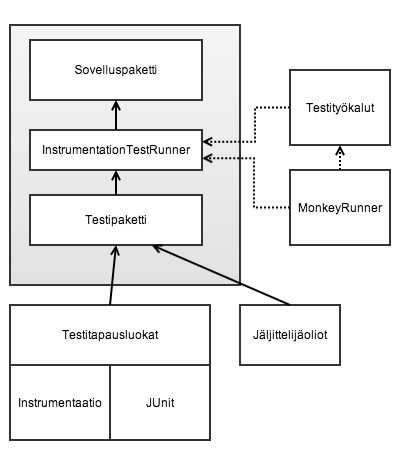
\includegraphics[width=100mm]{test_framework.png}
\caption{Android-testien ajoympäristö} \label{test_framework}
\end{figure}

Androidin-sovelluksen testejä voi ajaa joko emulaattorilla tai suoraan puhelimessa. Androidin testisarjat perustuvat JUnit-testikehikkoon. Puhdasta JUnitia voi käyttää sellaisen koodin testaamiseen, joka ei kutsu Androidin rajapintaa tai sitten voi käyttää Androidin JUnit-laajennusta Android-komponenttien testaukseen. Laajennus tarjoaa komponenttikohtaiset yliluokat testitapausten kirjoittamista varten. Nämä luokat tarjoavat apumetodeita jäljittelijöiden (mock object) luomiseen ja komponentin elinkaaren hallintaan. Androidin JUnit-toteutus mahdollistaa JUnitin versio 3:n mukaisen testityylin, ei uudempaa versio 4:n mukaista.

Kuvassa \ref{test_framework} on esitetty Androidin testien ajoympäristö. Testattavaa sovellusta testataan ajamalla testipaketissa olevat testitapaukset MonkeyRunnerilla (ks. luku \ref{monkeyrunner}). Testipaketti sisältää testitapausten lisäksi Androidin instrumentaatiota, eli apuvälineitä sovelluksen elinkaaren hallintaan ja koukkuja, joilla järjestelmän lähettämiä callback-metodikutsuja pääsee muokkaamaan, sekä jäljittelijäolioita korvaamaan järjestelmän oikeita luokkia testin ajaksi jäljittely-toteutuksella. \cite{android}

\subsection{Komponenttikohtaiset yksikkötestiluokat}

Android tarjoaa aktiviteeteille, palveluille ja sisällöntarjoajille jokaiselle oman testiyliluokkansa, joka mahdollistaa komponenttikohtaisten testien helpomman toteutuksen.

Aktiviteettien testauksessa Androidin JUnit-laajennus on merkittävä, koska aktiviteeteilla on monimutkainen elinkaari, joka perustuu paljolti takaisinkutsumetodeihin, joiden suora kutsuminen ei ole mahdollista. Aktiviteettien testauksen pääyliluokka on InstrumentationTestCase. Sen avulla on mahdollista käynnistää, pysäyttää ja tuhota testattavana oleva aktiviteetti halutuissa kohdissa. Lisäksi sen avulla voi jäljitellä järjestelmäolioita, kuten Context- ja Applications-luokan instansseja. Tämä mahdollistaa testin eristämisen muusta järjestelmästä ja aikeiden luomisen testejä varten. Lisäksi yliluokassa on metodit käyttäjän vuorovaikutusten, kuten kosketus- ja näppäimistötapahtumien lähettämiseen suoraan testattavalle luokalle.

Aktiviteettien testaamiseen on kaksi välitöntä yliluokkaa, ActivityUnitTestCase ja ActivityInstrumentationTestCase2. ActivityUnitTestCase on tarkoitettu luokan yksikkötestaamiseen siten, että se on eristetty Android-kirjastoista. Näitä testejä voi ajaa suoraan kehitystyökalu ja tarvittaessa Android-kirjaston mockaamiseen on käytössä MockApplication-olio. ActivityInstrumentationTestCase2 taas on tarkoitettu toiminnalliseen testaukseen tai useamman aktiviteetin testaamiseen. Ne ajetaan normaalissa suoritusympäristössä emulaattorilla tai Android-laitteessa. Aikeiden jäljittely on mahdollista, mutta testin eristäminen muusta järjestelmästä ei ole mahdollista.

Palveluiden testaaminen on paljon yksinkertaisempaa kuin aktiviteettien. Ne toimivat eristyksessä muusta järjestelmästä, joten testattaessakaan ei tarvita Androidin instrumentaatiota. Android tarjoaa ServiceTestCase-yliluokan palveluiden testaamiseen. Se tarjoaa jäljittelijäoliot Application- ja Context-luokille, joten palvelun saa testattua eristettynä muusta järjestelmästä. Testiluokka käynnistää testattavan palvelun vasta kutsuttaessa sen startService() tai bindService()-metodia, jolloin jäljittelijäoliot voi alustaa ennen palvelun käynnistymistä. Jäljittelijäolioiden käyttö palveluiden testaamisessa paljastaa myös mahdolliset huomaamatta jääneet riippuvuudet muuhun järjestelmään, koska Jäljittelijäoliot heittävät poikkeuksen, mikäli niihin tulee metodikutsu, johon ei ole varauduttu.

Sisällöntarjoajien testaaminen on erityisen tärkeää, jos sovellus tarjoaa sisällöntarjoajiaan muiden sovellusten käyttöön. Tällöin on myös olennaista testata niitä käyttäen samaa julkista rajapintaa, jota muut sovellukset joutuvat käyttämään kommunikoidessaan sisällöntarjoajien kanssa. Sisällöntarjoajien testauksen yliluokka on ProviderTestCase2, joka tarjoaa käyttöön jäljittelijäoliot ContentResolveriosta ja Contextista, jolloin sisällöntarjoajia voi testaja eristyksissä muusta sovelluksesta. Yliluokka tarjoaa myös metodit sovelluksen oikeuksien testaamisen. Contextin jäljittelijäolio mahdollistaa tiedosto- ja tietokantaoperaatiot, mutta muut Androidin kirjastokutsut on toteutettu tynkinä (stub). Lisäksi tiedon kirjoitusosoite on uniikki testissä, joten testien ajaminen ei yliaja varsinaista sovelluksen tallentamaa tietoa. Sisällöntarjoajatestit ajetaan emulaattorissa tai Android-laitteella. \cite{android}

\subsection{MonkeyRunner}
\label{monkeyrunner}

MonkeyRunner tarjoaa rajapinnan, jolla Android-sovellusta voi ohjata laitteessa tai emulaattorissa. Se on lähinnä tarkoitettu toiminnallisten testien sekä yksikkötestien ajamiseen, mutta soveltuu myös muihin tarkoituksiin. Sen avulla voi esimerkiksi asentaa sovelluksia, ajaa testisarjoja ja sovelluksia ja lähettää niihin syötteitä. Lisäksi monkeyrunnerilla voi ottaa eri kohdista kuvakaappauksia ja verrata niitä referenssikuviin. Tällä tavalla voidaan tehdä esimerkiksi regressiotestausta.

MonkeyRunnerilla voidaan testata yhtä aikaa monia eri emulaattoreita tai useita laitteita, jolloin voidaan tehdä fragmentaatiotestausta. MonkeyRunner on myös laajennettavissa, jolloin sitä voi käyttää muihinkin tarkoituksiin. MonkeyRunneria ohjataan pythonilla ja se on toteutettu jythonilla, joka on Javan virtuaalikoneessa pyörivä python-toteutus \cite{android}.

\subsection{Uiautomator ja Uiautomatorviewer}

Uiautomator tarjoaa mahdollisuuden kirjoittaa toiminnallisia mustalaatikko-testejä Android-sovelluksille Monkeyrunneria paremmat assert-mahdollisuudet ja mahdollisuuden toiminallisten musta laatikko -testien kirjoittamiseen Javalla tarjoaa Uiautomator. Siinä on kaksi komponenttia: Uiautomatorviewer ja Uiautomator. Uiautomatorviewer on graafinen työkalu, jolla voi analysoida ja skannata Android-sovelluksen käyttöliittymää ja Yiautomator työkalu, joka tarjoaa rajapinnan ja moottorin toiminnallisten mustalaatikkotestien ajamiseen.

\begin{figure}[htb]
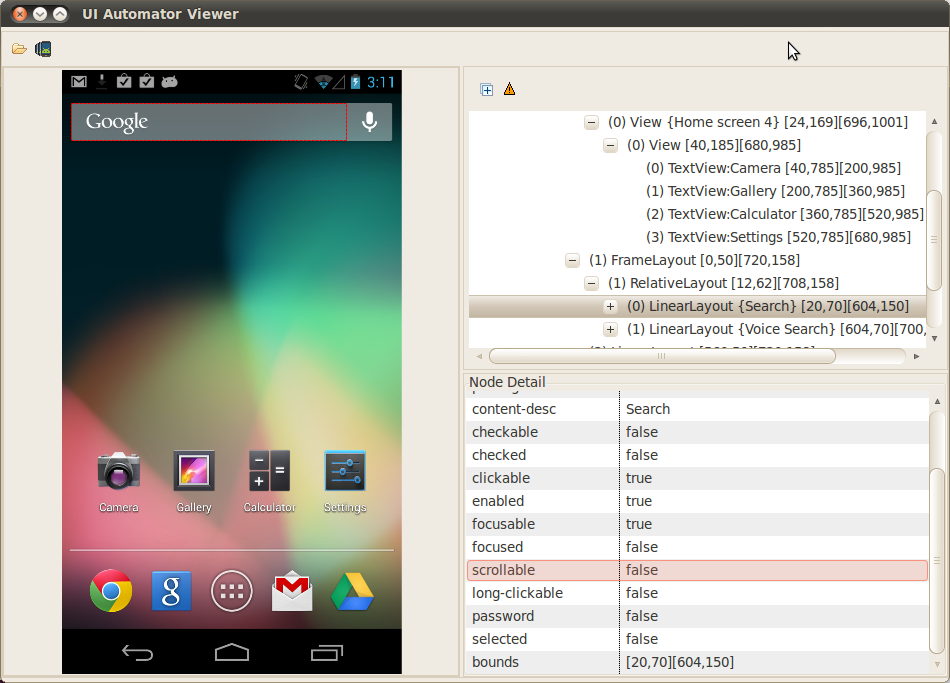
\includegraphics[width=160mm]{uiautomatorviewer.png}
\caption{UIAutomatorViewerin käyttöliittymä} \label{uiautomatorviewer}
\end{figure}

Uiautomatorviewer (kuvassa \ref{uiautomatorviewer}) analysoi sovelluksen näkymän komponentit. Vasemmalla näkymässä punaisella ympyröitynä on oikeasta valikosta valittu komponentti. Oikeassa alareunassa näytetään komponentin tietoja, joita voi käyttää testeissä esimerkiksi komponentin valitsijoissa, esimerkiksi siten, että valitaan save-nappi tekstin perusteella, jotta siitä voidaan testissä painaa.

Uiautomator-testit kirjoitetaan Javalla JUnitiin pohjautuen perimällä UIAutomatorTestCase-yliluokka, joka tarjoaa käyttöön käyttöliittymäelementtien valitsemiseen tarvittavan rajapinnan ja mahdollisuuden vuorovaikutukseen niiden kanssa. UISelector-luokassa on metodeita käyttöliittymäelementtien valitsemiseen ja UIObject-luokassa niiden kanssa kommunikointia varten. UIObject-oliolta voi kysyä assertointia varten elementin olemassaoloa ja erilaisia tilaan liittyviä tietoja, kuten onko elementti käytössä tai painettavissa.

Uiautomator on uusi työkalu ja testejä voi ajaa vain laitteilla, jotka tukevat API:n versiota 16 tai uudempaa. Tämä vastaa Androidin versiota 4.1, joka on julkaistu kesäkuussa 2012. Uiautomatorilla ei voi siis testata sovellusta vanhemmilla Android-laitteilla, joita on tällä hetkellä vielä reilusti yli puolet Androidin laitekannasta \cite{android}.

\subsection{Monkey}

Monkey on Androidin mukana tuleva työkalu, jota voi ajaa emulaattorissa tai Android-laitteessa ja joka tuottaa sovellukselle pseudosatunnaisia syötteitä. Näitä voi olla esimerkiksi painallukset, eleet sekä järjestelmätason viestit. Monkeytä voi käyttää esimerkiksi sovelluksen stressitestaukseen tai fuzz-testaukseen.

Monkeylle voi antaa jonkin verran sen toimintaa ohjaavia parametreja. Ensinnäkin testisyötteiden määrää ja tiheyttä voi rajoittaa. Toiseksi erityyppisten syötteiden osuutta voi säätää. Kolmanneksi testauksen voi rajoittaa tiettyyn pakettiin sovelluksessa. Tällöin Monkey pysäyttää testauksen, jos se on ajautuu muihin kuin haluttuun osaan sovelluksesta. Neljänneksi Monkeyn tulosteiden määrää ja tarkkuutta voi säätää.

Monkey pystäyttää testin, jos ohjelmasta lentää käsittelemätön poikkeus tai jos järjestelmä lähettää sovellus ei vastaa -virheviestin. Näissä tapauksissa Monkey antaa raportin virheestä ja miten se syntyi. Monkey voi myös tehdä profilointiraportin testistä.\cite{android}